\section{Signal and Backgroud processes}

This analysis aims at the VBS semi-leptonic process. The experimental characterization of the process and the Signal and backgroud (BG) processes are explained in this section.

\subsection{The characteristic of the VBS semi-leptonic process}
The experimental characteristic of the VBS process is described by two vector bosons in the central region and the two jets which go forward.
The kinematics of this process is illustrated in Figure~\ref{fig:VBStopology}.
\begin{figure}[tbp]
\begin{center}
%\subfigure[]{
 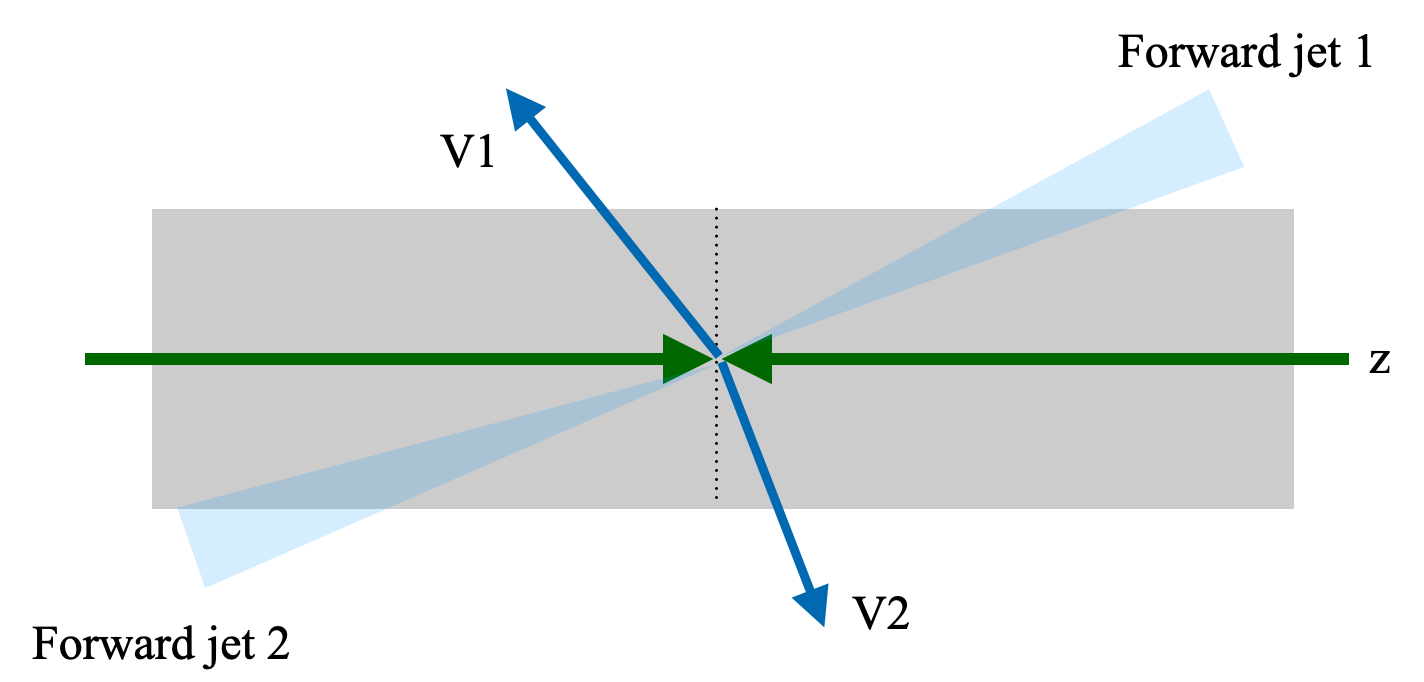
\includegraphics[width=0.75\textwidth,keepaspectratio]{figures/VBStopology}
%}
\caption{
The VBS topology
}
\label{fig:VBStopology}
\end{center}
\end{figure}

The forward jets are two small-R jets, tagged by requiring the highest invariant mass. The one boson are reconstructed by two small-R jets or one large-R jets, and the other boson are from leptons and/or missing $E_T$ ($E_T^{miss}$).

\subsection{Signal process}

The signals of this analysis are modeled as the electroweak (EWK) VV$\plus$jj production. The signal samples are generated with two on-shell V bosons, with one V boson decaying leptonically ($Z \rightarrow ll$ with $l = e,\mu$, $Z \rightarrow \nu\nu$, $W\rightarrow l\nu$ with $l = e,\mu,\tau$ ), and the other V boson decaying hadronically. The production cross sections of all types of signal samples are summarized in the Table~\ref{tab:VBS_sig_samples}. The decaying channel is devided into three considering the number of leptons as 0,1,2-lepton final states. 

\begin{table}[!htbp]
\begin{center}
\small
\begin{tabular}{|l|l|}
\hline
Process & cross-section~(pb) \\
\hline
$W(l\nu)W(qq\prime)jj,b-veto$     & 1.99    \\
$W(l\nu)W(qq\prime)jj,b-filter$   &  1.97   \\
$W(l\nu)Z(qq\prime)jj$            &  0.25   \\
$W(\nu\nu)W(qq\prime)jj$          &  0.15   \\
$Z(ll)W(qq\prime)jj$              &  0.045  \\
$Z(\nu\nu)Z(qq\prime)jj$          &  0.032  \\
$Z(ll)Z(qq\prime)jj$              &  0.0096 \\
\hline
\end{tabular}
\caption{List of VBS samples used in the analysis.
}
\label{tab:VBS_sig_samples}
\end{center}
\end{table}

The signal samples include all purely-electroweak tree-level diagrams:
\begin{itemize}
    \item \textbf{VBS diagrams} 
    \\ which includes the scatterings of two vector bosons, shown in Fig~\ref{fig:feynmanVBS}
    \item \textbf{non-VBS diagrams} 
    \\ which does not includes the scatterings of two vector bosons, shown in Fig~\ref{fig:feynmanEWKnonVBS}. The electroweak $t\bar{t}$ contriburion, which is shown in Figure~\ref{} has a significant contribution about~50-60\%, which can be reduced by applying b-veto. After b-veto is applied, theres is still non-negligible non-VBS contribution of tZb process, which is shown in Figure~\ref{}.This contributions are reduced by applying additional cut described in Section~\ref{}.
\end{itemize}

These VBS and non-VBS diagrams cannot be separate in production, since gauge invariant must be conserved. Therefore these non-VBS diagrams are also included in the signal samples.

The EWK VV+jj production is modeled using MadGraph5\_aMC@NLO v2.3.3~\cite{Alwall:2014hca},
plus \PYTHIA8~\cite{Sjostrand:2007gs} for fragmentation.
The \textsc{NNPDF30LO} PDF set~\cite{Ball:2012cx} is used.

%% feynman diagrams, VBS
\begin{figure}[tbp]
\begin{center}
 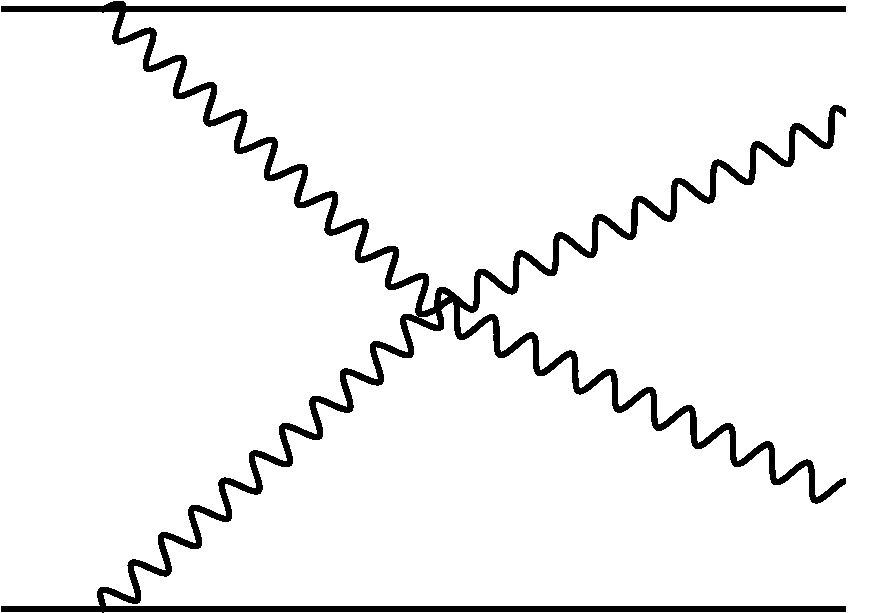
\includegraphics[width=0.3\textwidth,keepaspectratio]{figures/samples/feynVBS2.pdf}
 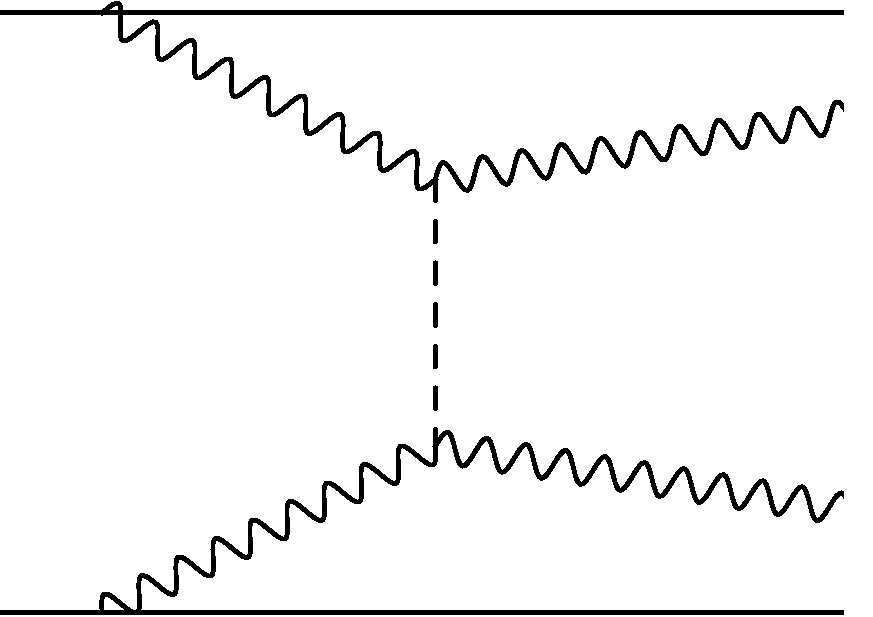
\includegraphics[width=0.3\textwidth,keepaspectratio]{figures/samples/feynVBS1.pdf}
 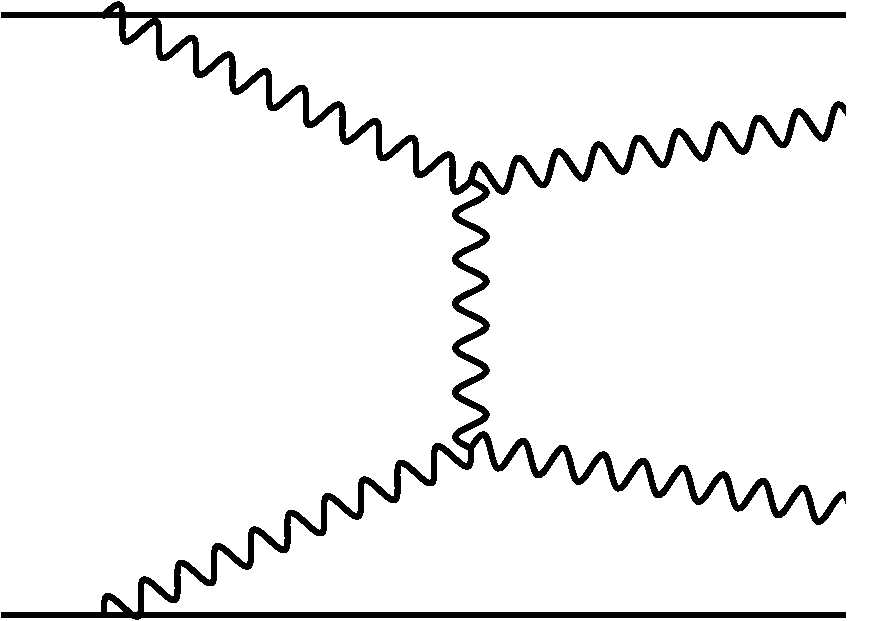
\includegraphics[width=0.3\textwidth,keepaspectratio]{figures/samples/feynVBS3.pdf}
 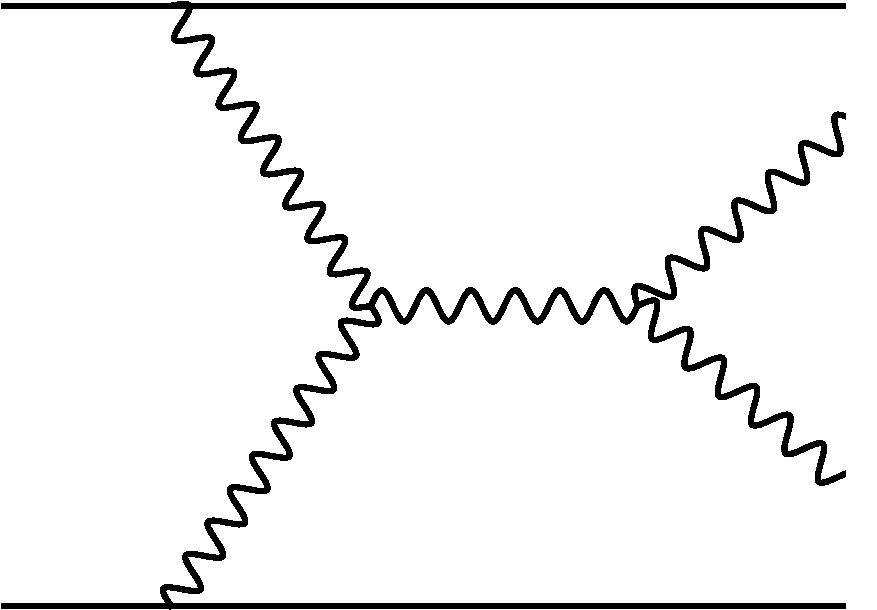
\includegraphics[width=0.3\textwidth,keepaspectratio]{figures/samples/feynVBS4.pdf}
 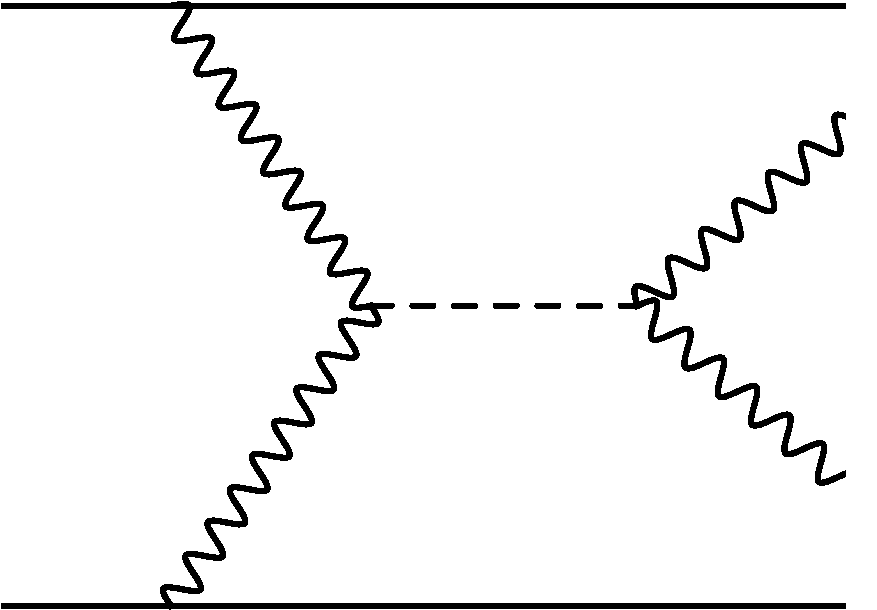
\includegraphics[width=0.3\textwidth,keepaspectratio]{figures/samples/feynVBS5.pdf}
\caption[f]{
VBS diagrams contribute to the signal.  
The dashed line represents the Higgs boson.The decays of the bosons are not shown.
}
\label{fig:feynmanVBS}
\end{center}
\end{figure}

%% feynman diagrams, non-VBS
\begin{figure}[tbp]
\begin{center}
 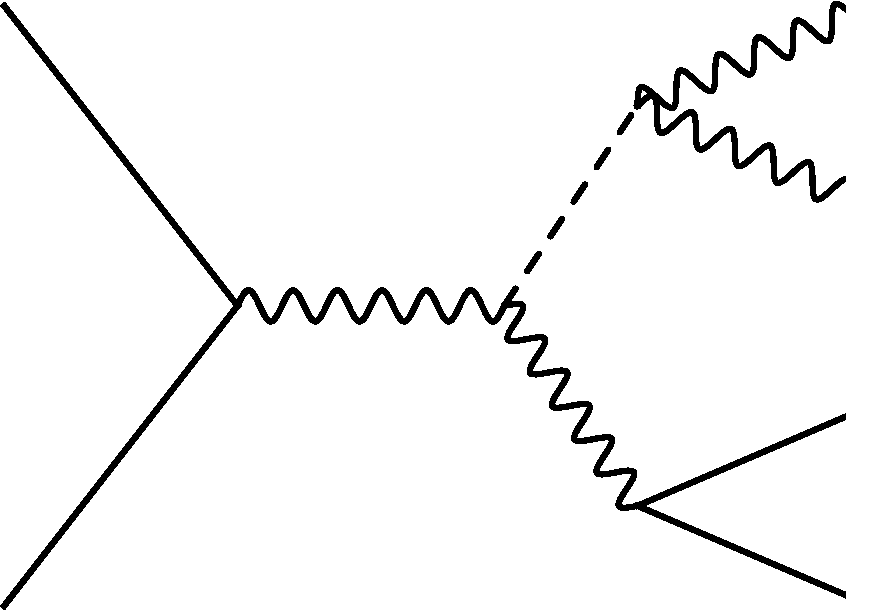
\includegraphics[width=0.25\textwidth,keepaspectratio]{figures/samples/feynEWKnonVBS3.pdf}
 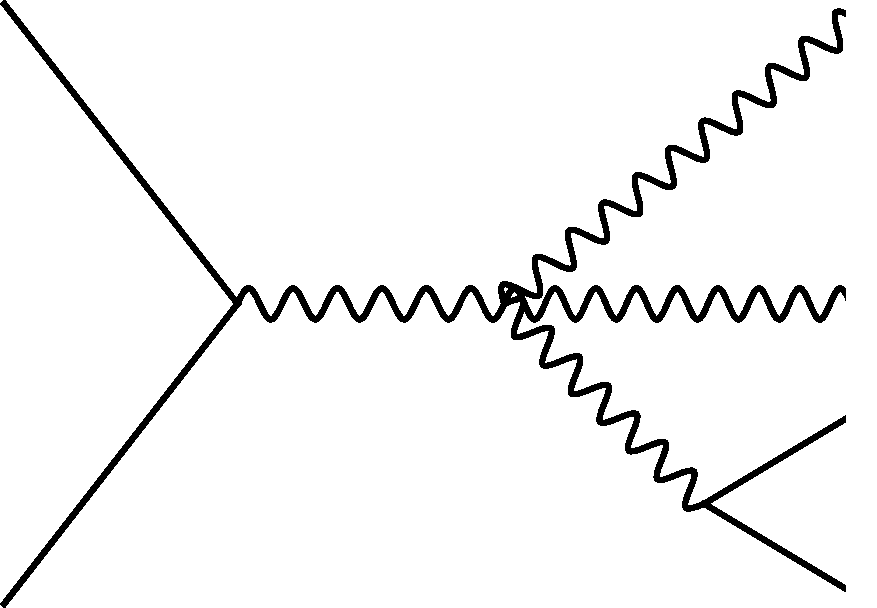
\includegraphics[width=0.25\textwidth,keepaspectratio]{figures/samples/feynEWKnonVBS4.pdf}
 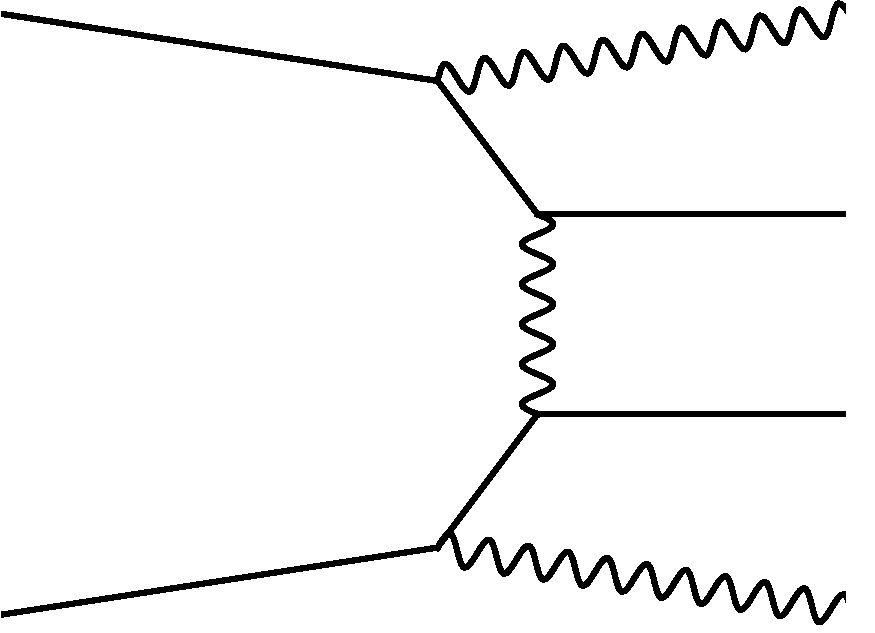
\includegraphics[width=0.25\textwidth,keepaspectratio]{figures/samples/feynEWKnonVBS5.pdf}
 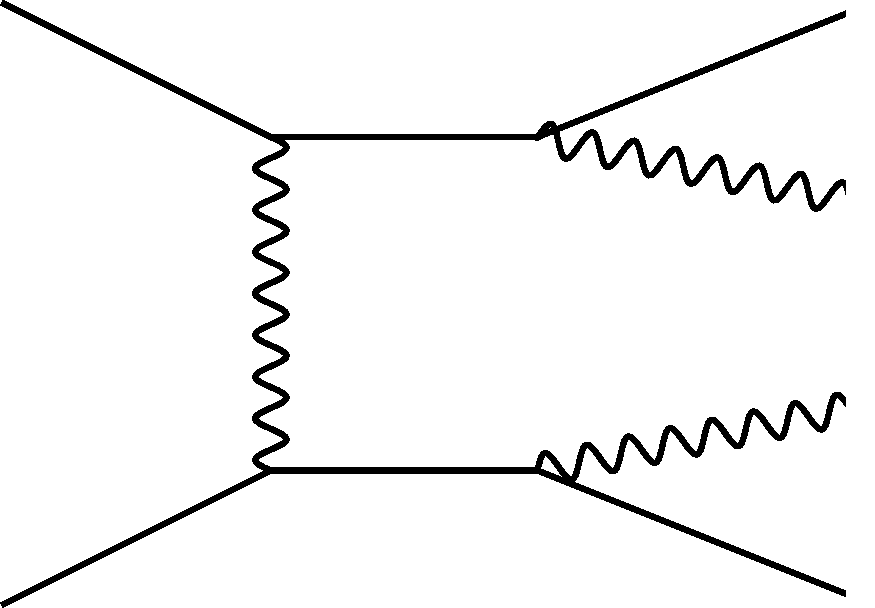
\includegraphics[width=0.25\textwidth,keepaspectratio]{figures/samples/feynEWKnonVBS6.pdf}
 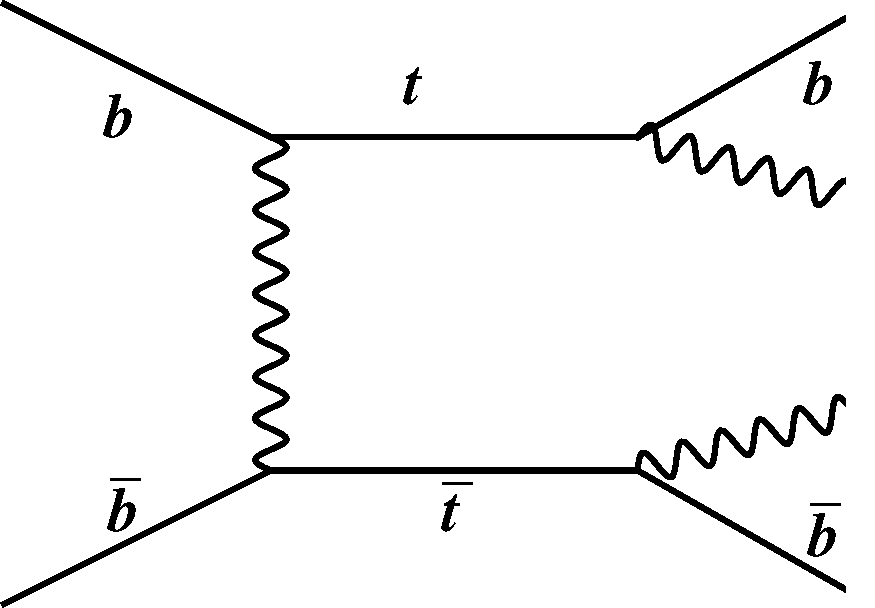
\includegraphics[width=0.3\textwidth,keepaspectratio]{figures/samples/feynEWKnonVBS1.pdf}
 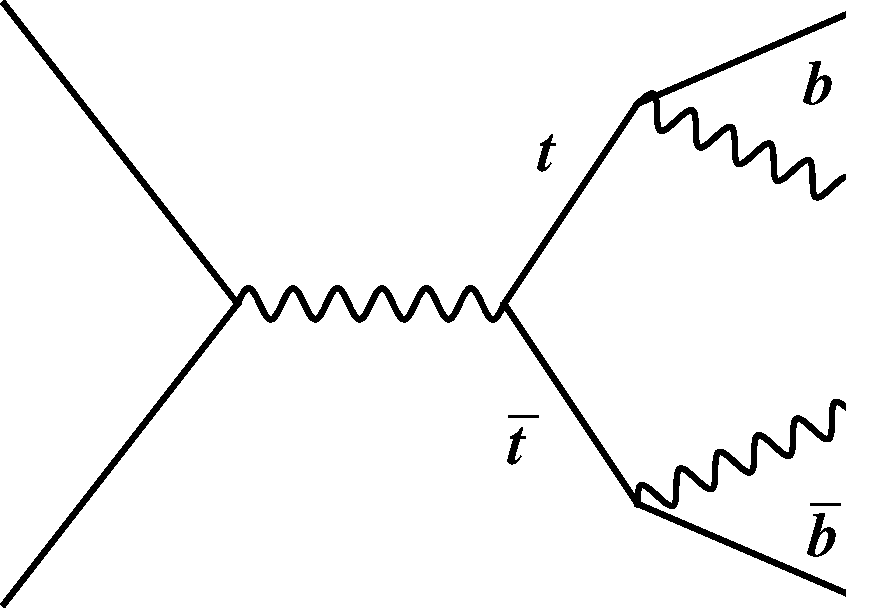
\includegraphics[width=0.3\textwidth,keepaspectratio]{figures/samples/feynEWKnonVBS2.pdf}
 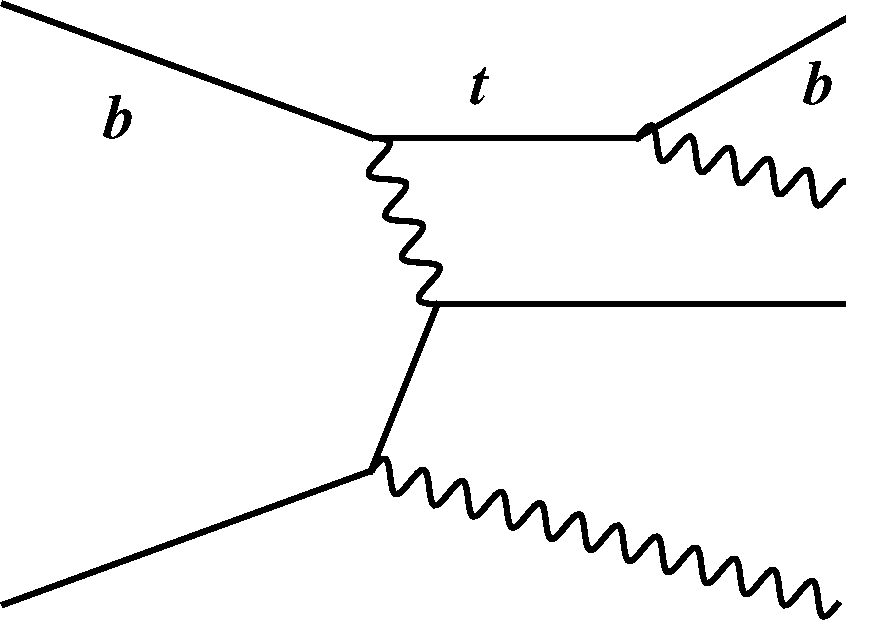
\includegraphics[width=0.3\textwidth,keepaspectratio]{figures/samples/feynEWKnonVBS7.pdf}
\label{fig:feynmanEWKnonVBS}
\end{center}
\end{figure}

%% feynman diagram, tZb
\begin{figure}[tbp]
\begin{center}
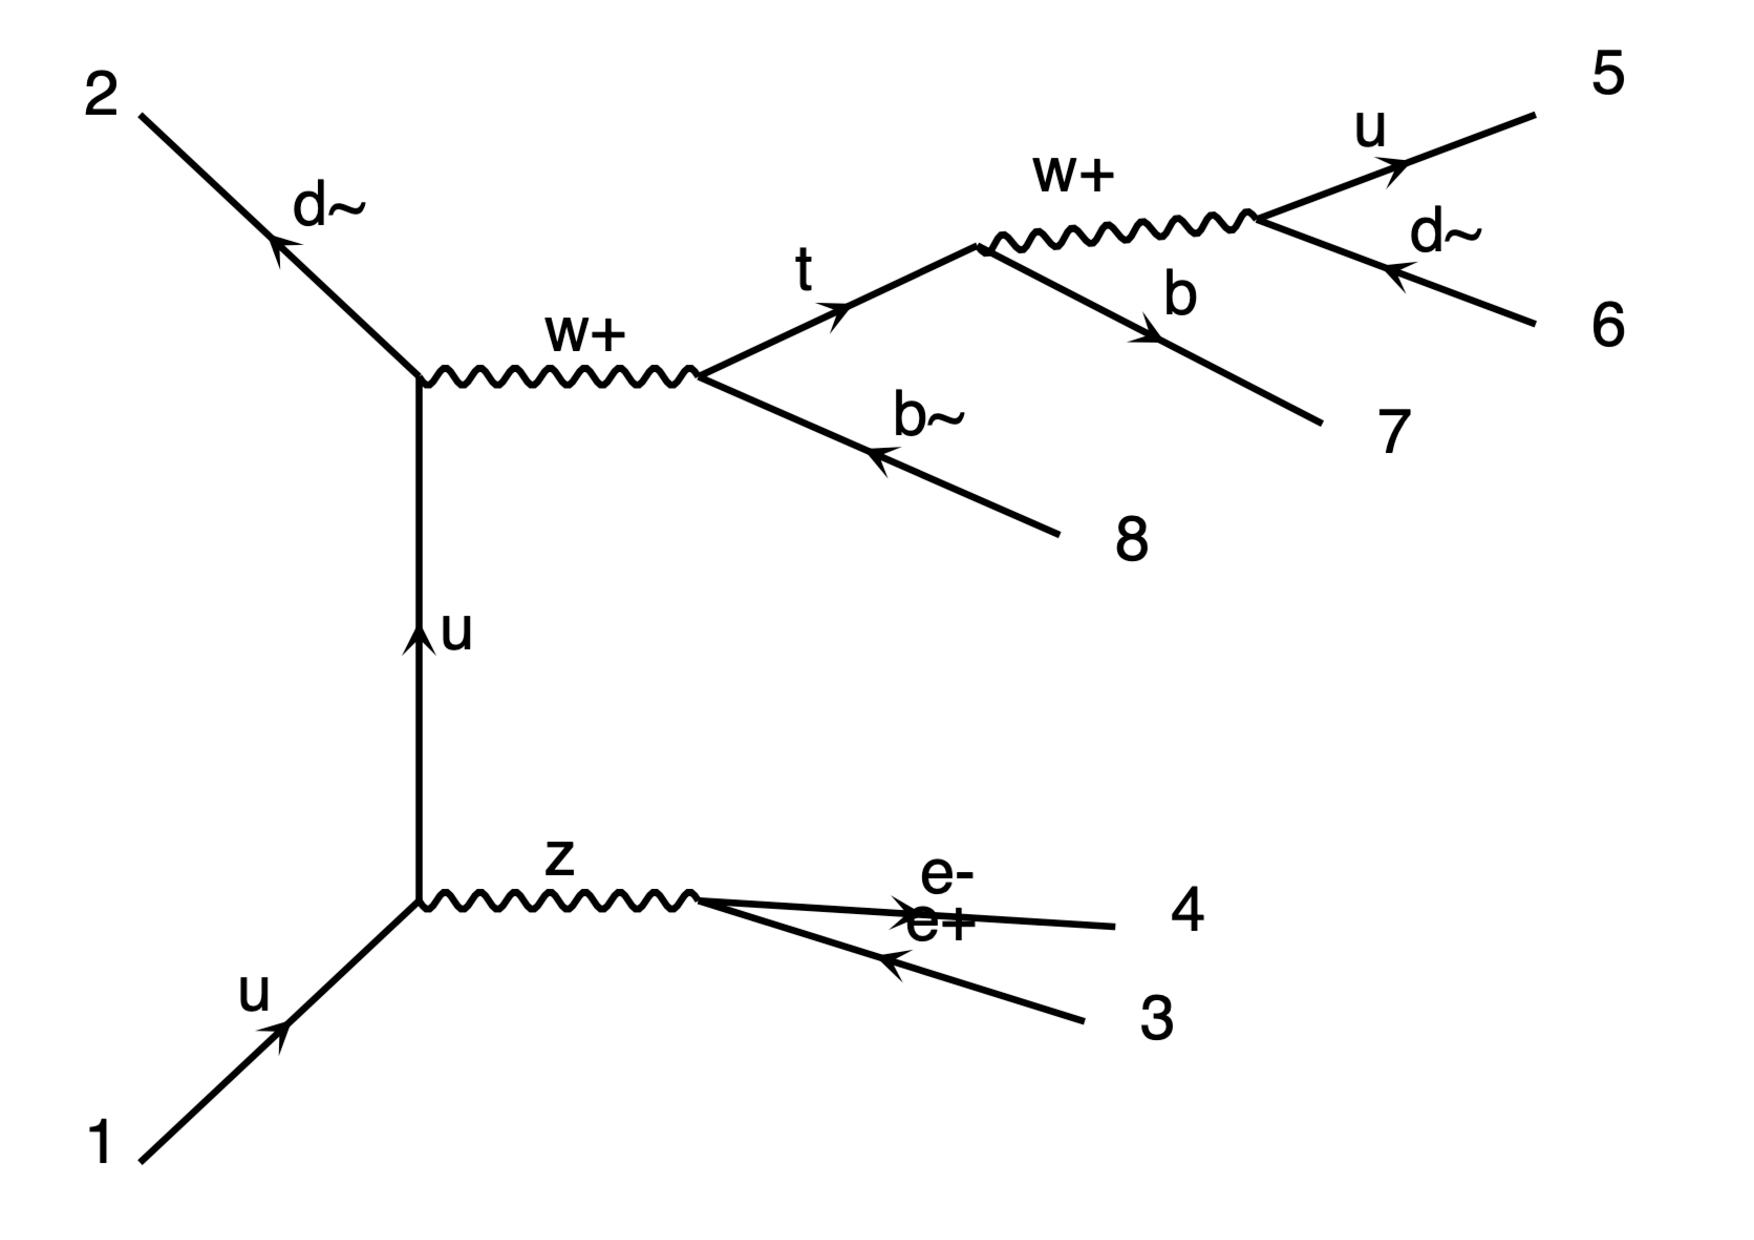
\includegraphics[width=0.5\textwidth,keepaspectratio]{figures/samples/feynEWKnonVBStZb.pdf}
\caption{
The example of the tZb diagram, which included in non-VBS $\mathcal{O}(\alpha_{EW}^6)$ diagrams.
}
\label{fig:feynmantZb}
\end{center}
\end{figure}

\subsection{Background process}

The Background processes for this process is  $W$/$Z$ $\plus$ jets, $t\bar{t}$, single top, diboson (WW,WZ,ZZ) and multi-jets productions. 

The main background for this analysis is the  $W$/$Z$ $\plus$ jets, which is the single W or Z boson in associated with jets. The V $\plus$ jets are modeled using Sherpa~2.2.1~\cite{Gleisberg:2008ta} generator. Matrix element is calculated for up to 2 partons at NLO, and 4 partons at LO using the Comix~\cite{Gleisberg:2008fv} and OpenLoops\cite{Cascioli:2011va}. Matrix element generators and merged with the Sherpa parton shower~\cite{Schumann:2007mg} using the ME+PS@NLO prescription~\cite{Hoeche:2012yf}.The NNPDF3.0NNLO PDF set is used in association to authors' tuning.The $W$/$Z$ + jets events are normalized to the NNLO cross sections.

The $t\bar{t}$ and single-top events are generated with the Powheg-Box~\cite{Alioli:2010xd} generator with the \\
NNPDF3.0NLO PDF\cite{Ball:2014uwa} sets in the matrix element calculation.
The top quark spin correlations are preserved (for t-channel, top quarks are decayed using MadSpin~\cite{Artoisenet:2012st}).
For all processes the parton shower, fragmentation, and the underlying event are simulated using \textsc{Pythia}8.230 with the A14 tune set\cite{ATL-PHYS-PUB-2014-021}.
The top mass is set to $172.5\gev$.
The cross sections of $t\bar{t}$ and single-top are known to NNLO in QCD including re-summation of next-to-next-to-leading logarithmic (NNLL) soft gluon terms\cite{Czakon:2011xx,Kidonakis:2011wy,Kidonakis:2010tc,Kidonakis:2010ux}.
The parameter \textsc{Hdamp} to regulate the high-\pt\ radiation in the \textsc{Powheg} is set to $1.5m_{t}$ for a good data/MC agreement at high \pt\ region\cite{ATL-PHYS-PUB-2016-020}.

The diboson processes ($WW$, $WZ$ and $ZZ$) are generated with Sherpa 2.2.1~\cite{Gleisberg:2008ta} generator.

The Signal and the Background processes are simulated by various Monte Carlo (MC) generators as previously described. 
All simulated events are processed with the same trigger and reconstruction algorithm as the data.The EvtGen v1.2.0 program~\cite{Lange:2001uf} is used for properties of the bottom and charm hadron decays.
Additional $pp$ collisions generated with \textsc{Pythia}~8.186\cite{Sjostrand:2008vc} are overlaid to model the effect of the pileup for all MC events.
Samples are processed through the full ATLAS detector simulation\cite{SOFT-2010-01} based on \textsc{GEANT4}\cite{Agostinelli:2002hh}.
All simulated events are processed with the same trigger and reconstruction algorithm as the data.

\subsection{Data sets}

\begin{table}[htb!p]
%\caption{An integrated luminosity used in this analysis. }
\label{tab:intLumi}
\begin{center}
\begin{tabular}{|l|l|}
\hline
Year & $\mathcal{L}$ [fb$^{-1}$] \\
\hline\hline
2015 & 3.21 \\
\hline
2016 & 32.88 \\
\hline
2017 & 44.31 \\
\hline
%2018 & 59.94 (21) for $\ell\nu qq$/$\ell\ell qq$ ($\nu\nu qq$) channel \\
     %& (will be updated to 58.45 with the latest lumi-tag) \\
2018 & 58.45 \\
\hline\hline
total & $139.0 \pm 2.4$ \\
\hline
\end{tabular}
\end{center}
\caption{An integrated luminosity used in this analysis. }
\end{table}




